\section{Research Methodology}

\subsection{Research Design}

This study follows the Design Science Research (DSR) approach. DSR is a research methodology that focuses on designing and developing practical solutions (artifacts) to solve real-world problems. It is commonly used in information systems and business analytics research where the goal is not only to analyze a problem but also to create and evaluate a solution. 

In this study, the artifact is a prescriptive decision-support framework that integrates demand forecasting and profit optimization for third-party delivery platforms. The DSR approach ensures that the framework is both theoretically grounded and practically useful.


\subsection{Design Science Research Process}

\begin{table}[h]
\centering
\begin{tabular}{|p{4cm}|p{10cm}|}
\hline
\textbf{DSR Step} & \textbf{Description} \\
\hline
Problem Identification & The problem is that HungryHub Oy has access to large amounts of sales data from platforms like Wolt and Foodora, but this data is not fully used for forecasting or decision-making. As a result, decisions are not fully data-driven and may lead to suboptimal outcomes. \\
\hline
Artifact Design & A decision-support framework is designed to address the problem. The framework includes data integration, demand forecasting, and profit optimization to transform raw sales data into actionable insights and recommendations. \\
\hline
Demonstration & The framework is applied to real historical sales data from Wolt and Foodora. Forecasting models are developed, and the results are used to generate decision recommendations. \\
\hline
Evaluation & The effectiveness of the framework is evaluated using forecasting accuracy metrics such as MAE, RMSE, or MAPE. In addition, simulation or back-testing is used to assess its potential impact on business performance. \\
\hline
\end{tabular}
\caption{Design Science Research (DSR) Process}
\end{table}

\subsection{System Architecture}
This proposed system architecture enables the data-driven decision making of third party delivery sales within the HungryHub Oy. The framework combines the data from Wolt or Foodora with an analysis and forecasting part in order to provide business insights and aid managerial decision making. The overall architecture of the proposed system is shown in Figure \ref{fig:architecture}. The architecture has five layers: Data sources, Data processing, Analytics and modeling, Application layer, Users. Business data is gathered and maintained in a central data repository from delivery platforms and/or internal business records. The data is then cleaned and integrated to be analyzed. The analytics layer consists of exploratory data analysis, demand forecasting and a profit-based decision model. The analysis of historical sales data is used to identify trends and forecast the need for future products. Forecasts generated are used for decision making and assessing business potential. Application layer offers dashboards and reporting tools, which visually present key performance indicators, predictions of outcomes and platform performance. It is designed to be used by management, operational personnel and data analysts for strategic and operational planning. In this study the framework is tested with historical data, but the proposed architecture can be used as a prototype for future real-time application.

\begin{figure}[h]
\centering
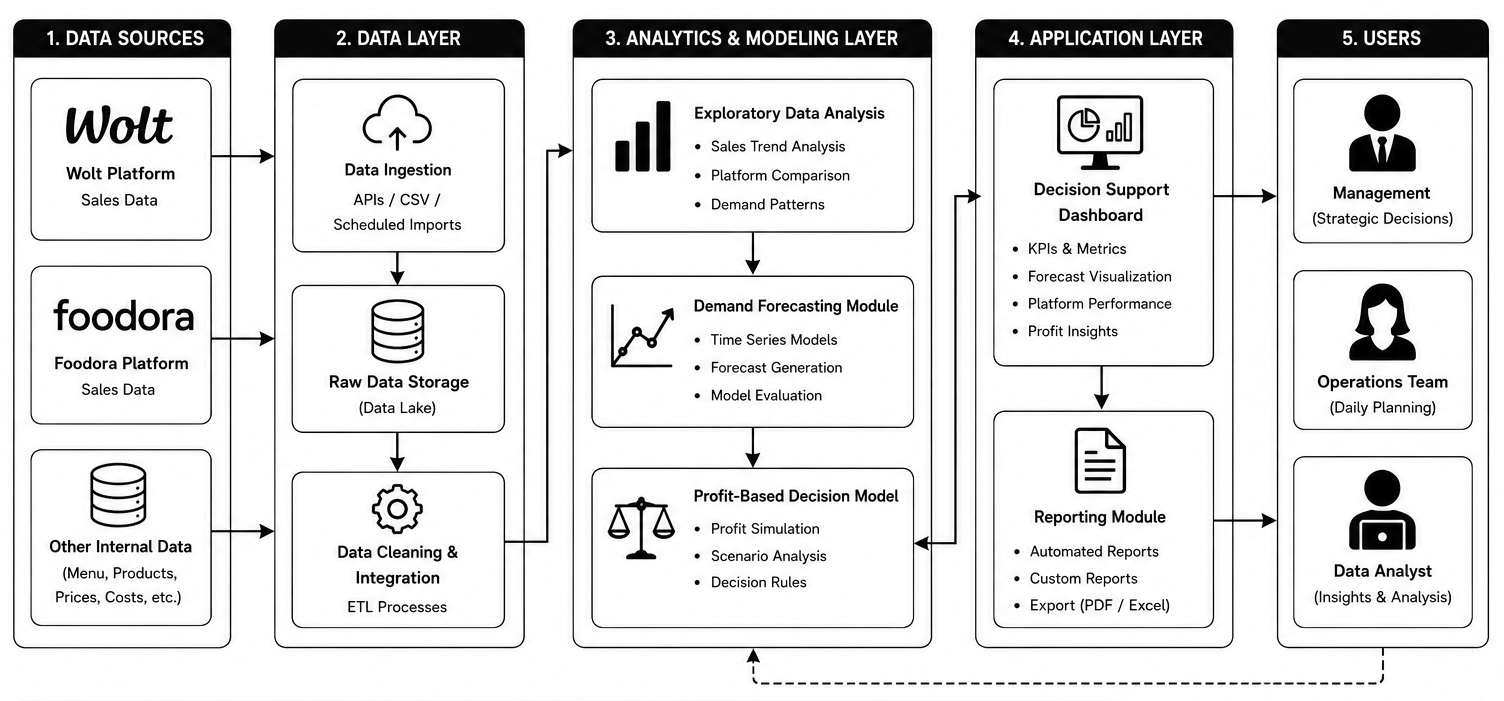
\includegraphics[width=\textwidth]{figures/System_Architecture.png}
\caption{System Architecture of the Proposed Data-Driven Decision Support Framework for Third-Party Delivery Sales}
\label{fig:architecture}
\end{figure}

\subsection{Data Collection}

This research employs historical sales data sourced from two third-party delivery platforms, specifically Wolt and Foodora. This includes transactional level data to understand the ordering trend, sales and demand at a platform level. These datasets are the building blocks for data analysis, prediction, and decision-support model creation.

\textbf{Wolt Dataset}

The Wolt data is from the historic sales records of wolt site. It includes data such as order date and time, sales value, and other relevant transaction data. Using this data we analyze demand behavior over time and build forecasting models at the platform level.

\textbf{Foodora Dataset}

Foodora also has the history of sale transactions data of the same type. Foodora platform. It provides information on when orders were placed, how many were sold and what features are important. This data is used alongside Wolt data for comparison and analysis, and to develop a joint forecasting and decision-support framework.


\subsection{Data Preprocessing}

The collected data needs to be preprocessed before analysis and model development to ensure accuracy and consistency. This step aims to improve data quality and prepare it for forecasting and optimization, so data preprocessing is an essential step.

\textbf{Data Cleaning}

Data cleaning is the processes of detecting and correcting (or removing) corrupt or inaccurate records from the dataset. It is about missing values, removing duplicate records and correcting the almost accurate records. Cleaning ensures the data is reliable and does not hold a bias towards model performance.

\textbf{Data Integration}

Data integration is the union of datasets that are given through more than one sources into one coherent single dataset. Since in this work sales info about Wolt and Foodora is going to be merged together to a single dataset. This allows for a consistent analysis across platforms and enables the construction of an overall forecasting- and decision support model.

\textbf{Feature Engineering}

Feature engineering is creating new ones or modifying existing ones to improve model performance. Examples Include features based on time as day of the week or month and hence extract features lag variables or computes sales sums. These features allow forecasting models to be more predictive and better capture the nature of patterns.

\subsection{Mathematical Formulation}
The mathematical formulations in this study are used to support the demand forecasting and the decision-making for profit in the proposed framework. Mathematical modeling can be used to provide a structured representation of sales behavior, forecasting performance, and profitability of a business \citep{botchkarev2018performanc}. These formulations offer a quantitative basis to analyse historical sales data from third-party delivery platforms. In the forecasting aspect of the study, it is assumed that future sales demands can be predicted from past sales pattern. The general forecasting function is represented as:
\begin{equation}
\hat{Y}_t = f(X_t)
\end{equation}

where $\hat{Y}_t$ represents the predicted sales value at time $t$, and $X_t$ is the historical sales observations and related variables used as input for the forecasting model. The purpose of the forecasting process is to recognize trends and recurring demand patterns from past transactions. To be able to forecast future sales. Sales demand can be further represented with trend, seasonal and irregular components (time-series behavior).:
\begin{equation}
Y_t = T_t + S_t + E_t
\end{equation}

where $Y_t$ represents the observed sales value at time $t$, $T_t$ is the long-term trend component, $S_t$ denotes seasonal variations, and $E_t$ indicates the random error component. This formulation supports the analysis of periodic demand fluctuations commonly observed in restaurant sales and food delivery platforms \citep{chai2014rooc}. In addition to forecasting, the framework includes a profit-oriented
decision model. The general profit equation is expressed as:
\begin{equation}
P = R - C
\end{equation}
where $P$ represents total profit, $R$ is called revenue generated from sales, and $C$ is the operational costs.
The objective of this formulation is to evaluate how forecasted sales demand may influence business profitability and managerial decision-making. The profit formulation can be extended to include item-level sales
performance:

\begin{equation}
P = \sum_{i=1}^{n}(S_i \times M_i) - C
\end{equation}

where $S_i$ denotes the sales volume of item $i$,
$M_i$ denotes the profit margin associated with item $i$,
and $C$ refers to total operational costs. This formulation enables the evaluation of product-level profitability and supports data-driven sales optimization.
To assess forecasting accuracy, evaluation metrics are incorporated into the framework. One commonly used metric is Mean Absolute Error (MAE), which measures the average prediction error:
\begin{equation}
MAE = \frac{1}{n}\sum_{i=1}^{n}\left|Y_i - \hat{Y}_i\right|
\end{equation}

where $Y_i$ represents the actual sales value and $\hat{Y}_i$ represents the predicted sales value. Lower MAE values indicate higher forecasting accuracy. Another important metric is Root Mean Square Error (RMSE), defined as:
\begin{equation}
RMSE = \sqrt{\frac{1}{n}\sum_{i=1}^{n}(Y_i - \hat{Y}_i)^2}
\end{equation}

RMSE measures the square root of the average squared forecasting error and gives greater importance to larger prediction deviations \citep{hodson2022root}. These evaluation metrics provide a systematic approach for comparing forecasting performance and validating the effectiveness of the proposed
analytical framework.

\subsection{Analytical Framework}

The research is based on a systematic analysis procedure which converts raw sales information into actionable decision support. The framework comprises of four key steps: data integration, descriptive analysis, predicting, and optimization.

The first step involves data integration whereby sales data of Wolt and Foodora are integrated into a.
single unified dataset. This makes it consistent and it can be analyzed on a number of platforms. Second, descriptive analysis is done to comprehend past sales trends. This involves finding trends, seasonal factors and platform differences. The objective of this step is to learn about the previous performance and to prepare the data to.
forecasting.

Third, there are forecasting models which are formulated to forecast future demand at the platform level. Various time series and machine learning methods are used and tested to identify maximize the best model. The basis of decision-making is based on these forecasts.
Lastly, optimization will be used to produce profit-oriented recommendations. Using the predicted demand, a decision model is created to aid in activities like platform level allocation or promotion planning.

This is where predictions are converted into actionable decisions which are meant to add value to business performance. In general, this analytical framework ties data, models and decisions into one process, allowing a shift in data analysis to data-driven decision-making..


\begin{figure}[h]
\centering
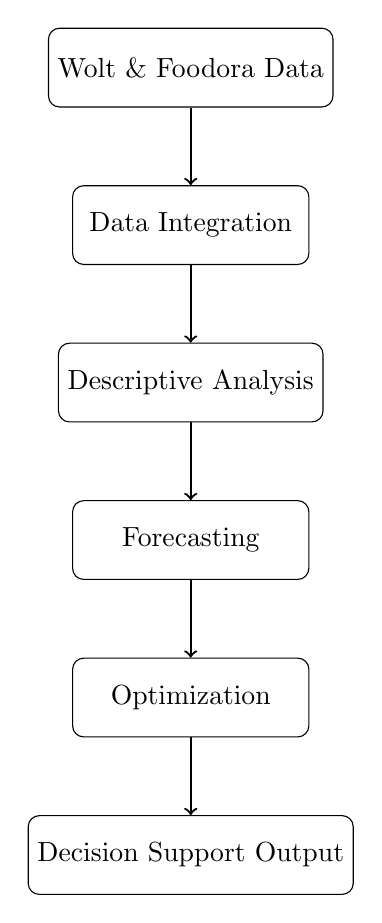
\begin{tikzpicture}[
    node distance=2cm,
    every node/.style={draw, rectangle, rounded corners, align=center, minimum width=3cm, minimum height=1cm},
    arrow/.style={->, thick}
]

\node (data) {Wolt \& Foodora Data};
\node (integration) [below of=data] {Data Integration};
\node (descriptive) [below of=integration] {Descriptive Analysis};
\node (forecasting) [below of=descriptive] {Forecasting};
\node (optimization) [below of=forecasting] {Optimization};
\node (decision) [below of=optimization] {Decision Support Output};

\draw[arrow] (data) -- (integration);
\draw[arrow] (integration) -- (descriptive);
\draw[arrow] (descriptive) -- (forecasting);
\draw[arrow] (forecasting) -- (optimization);
\draw[arrow] (optimization) -- (decision);

\end{tikzpicture}
\caption{Analytical Framework of the Study}
\end{figure}